%- block legend
Kurt, o camaleão (Mascote do PPCI) é um colecionador de relógios antigos. Ele possui $N$ relógios, cada um marcando uma hora diferente em mostradores de 12 horas, com ponteiros de horas, minutos e segundos. 

Kurt descobriu um botão curioso em cada relógio: ao pressionar o botão em um relógio específico, todos os outros relógios (exceto o pressionado) adiantam exatamente um segundo. 

Por exemplo, se há três relógios marcando:

\begin{center}
\texttt{[01:00:00, 03:00:00, 05:00:00]}
\end{center}
e Kurt pressiona o botão do segundo relógio (03:00:00), o resultado será:
\begin{center}
\texttt{[01:00:01, 03:00:00, 05:00:01]}
\end{center}

Kurt deseja que todos os relógios mostrem exatamente a mesma hora (mesmo valor de horas, minutos e segundos).  
Determine o número mínimo de vezes que ele precisa apertar algum botão para que isso aconteça.

Os relógios operam em formato de 12 horas, isto é, após \texttt{11:59:59} vem \texttt{00:00:00} novamente.
%- endblock

%- block input
A primeira linha contém um inteiro $N$ ($1 \leq N \leq 10^5$), o número de relógios.  

Cada uma das próximas $N$ linhas contém três inteiros $h_i$, $m_i$ e $s_i$ ($0 \le h_i \le 11$, $0 \le m_i, s_i \le 59$), representando a hora, minuto e segundo mostrados no $i$-ésimo relógio.
%- endblock

%- block output
Imprima um único inteiro, o número mínimo de vezes que Kurt precisa pressionar algum botão para que todos os relógios fiquem iguais.
%- endblock

%- block notes
No primeiro caso teste como só há apenas $2$ relógios: 

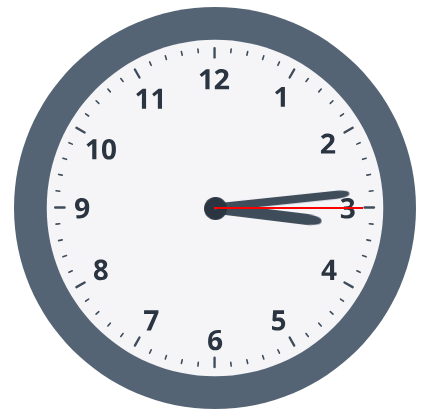
\includegraphics[scale=0.35]{relogio1.png}
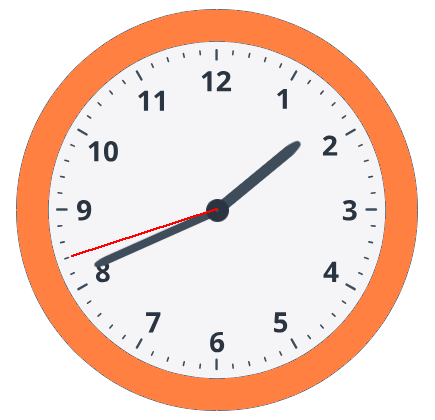
\includegraphics[scale=0.35]{relogio3.png}

Kurt pode apertar o botão do primeiro relógio até que o segundo fique sincronizado com ele, o que ocorre após 5553 cliques:

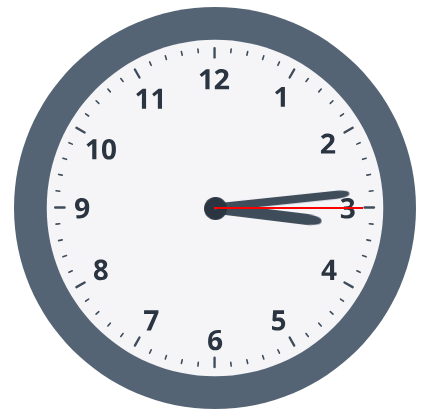
\includegraphics[scale=0.35]{relogio1.png}
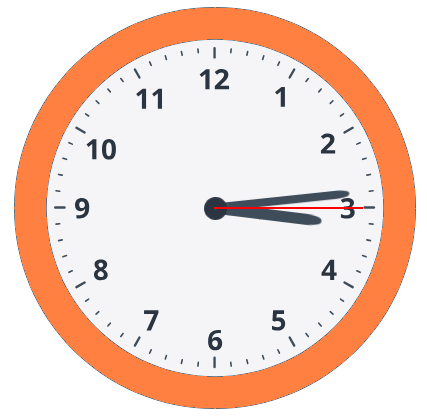
\includegraphics[scale=0.35]{relogio2.png}
%- endblock

%- block editorial
teste
%- endblock
